
All four hypotheses passed their gate conditions.

\subsubsection{H-E1: Inter-Benchmark Correlations}

Cross-benchmark correlations fall in the moderate range:

\begin{table*}[htbp]
\centering
\resizebox{\dimexpr 2\columnwidth+\columnsep\relax}{!}{%
\begin{tabular}{lllll}
\toprule
Benchmark Pair & Spearman r & 95\% CI & p-value (adj) & Gate \\
\midrule
TruthfulQA--HaluEval & 0.58 & [0.36, 0.74] & 3.$3\times 10^{-5}$ & PASS \\
TruthfulQA--FactScore & 0.42 & [0.16, 0.63] & 0.0065 & PASS \\
HaluEval--FactScore & 0.44 & [0.19, 0.64] & 0.0037 & PASS \\
\bottomrule
\end{tabular}
}
\end{table*}

Baseline reference: r(MMLU-Physics, HaluEval) = 0.10

All correlations satisfy the gate condition: 0.10 < r < 0.70. All p-values are significant after Bonferroni correction (p < 0.0167).

\begin{figure}[htbp]
\centering
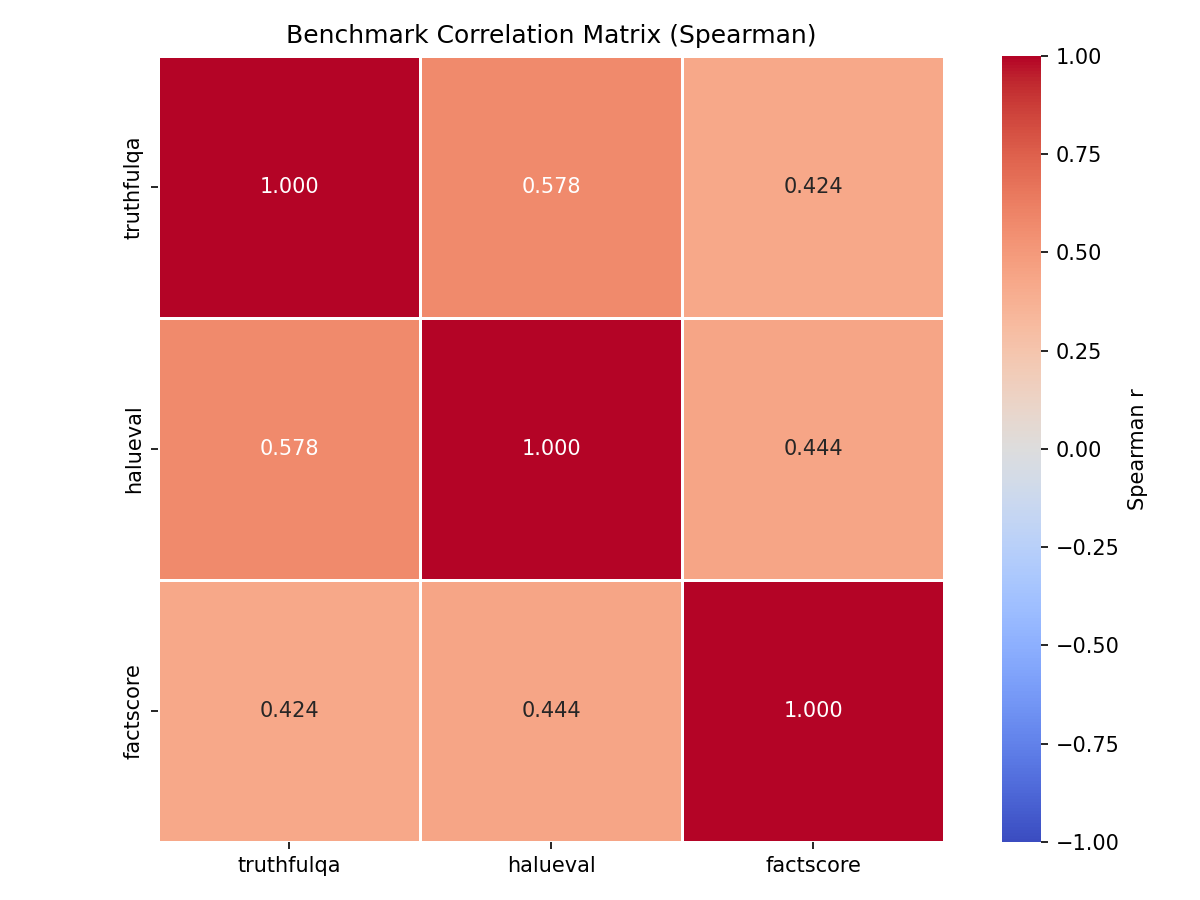
\includegraphics[width=\columnwidth]{figures/heatmap.png}
\caption{Correlation Heatmap}
\label{fig:heatmap}
\end{figure}

\subsubsection{H-M1: TruthfulQA vs. MMLU Distinctness}

TruthfulQA measures a capability distinct from general knowledge:

\begin{table}[htbp]
\centering
\resizebox{\columnwidth}{!}{%
\begin{tabular}{lll}
\toprule
Metric & Value & 95\% CI \\
\midrule
r(TruthfulQA, MMLU) & 0.19 & Not significant (p=0.19) \\
r(MMLU internal, mean) & 0.78 & --- \\
$r^2$ gap & 0.58 & --- \\
\bottomrule
\end{tabular}
}
\end{table}

The correlation between TruthfulQA and MMLU (r=0.19) is substantially lower than internal correlation among MMLU subjects (r=0.78), passing the gate condition.

\textbf{Divergent Profile Models:} Four models (8\%) exhibit high MMLU (z > 1.0) but low TruthfulQA (z < 0):
\begin{itemize}
\item yi-13b-instruct
\item qwen-70b-dpo
\item qwen-13b-instruct
\item llama-70b-dpo
\end{itemize}

\begin{figure}[htbp]
\centering
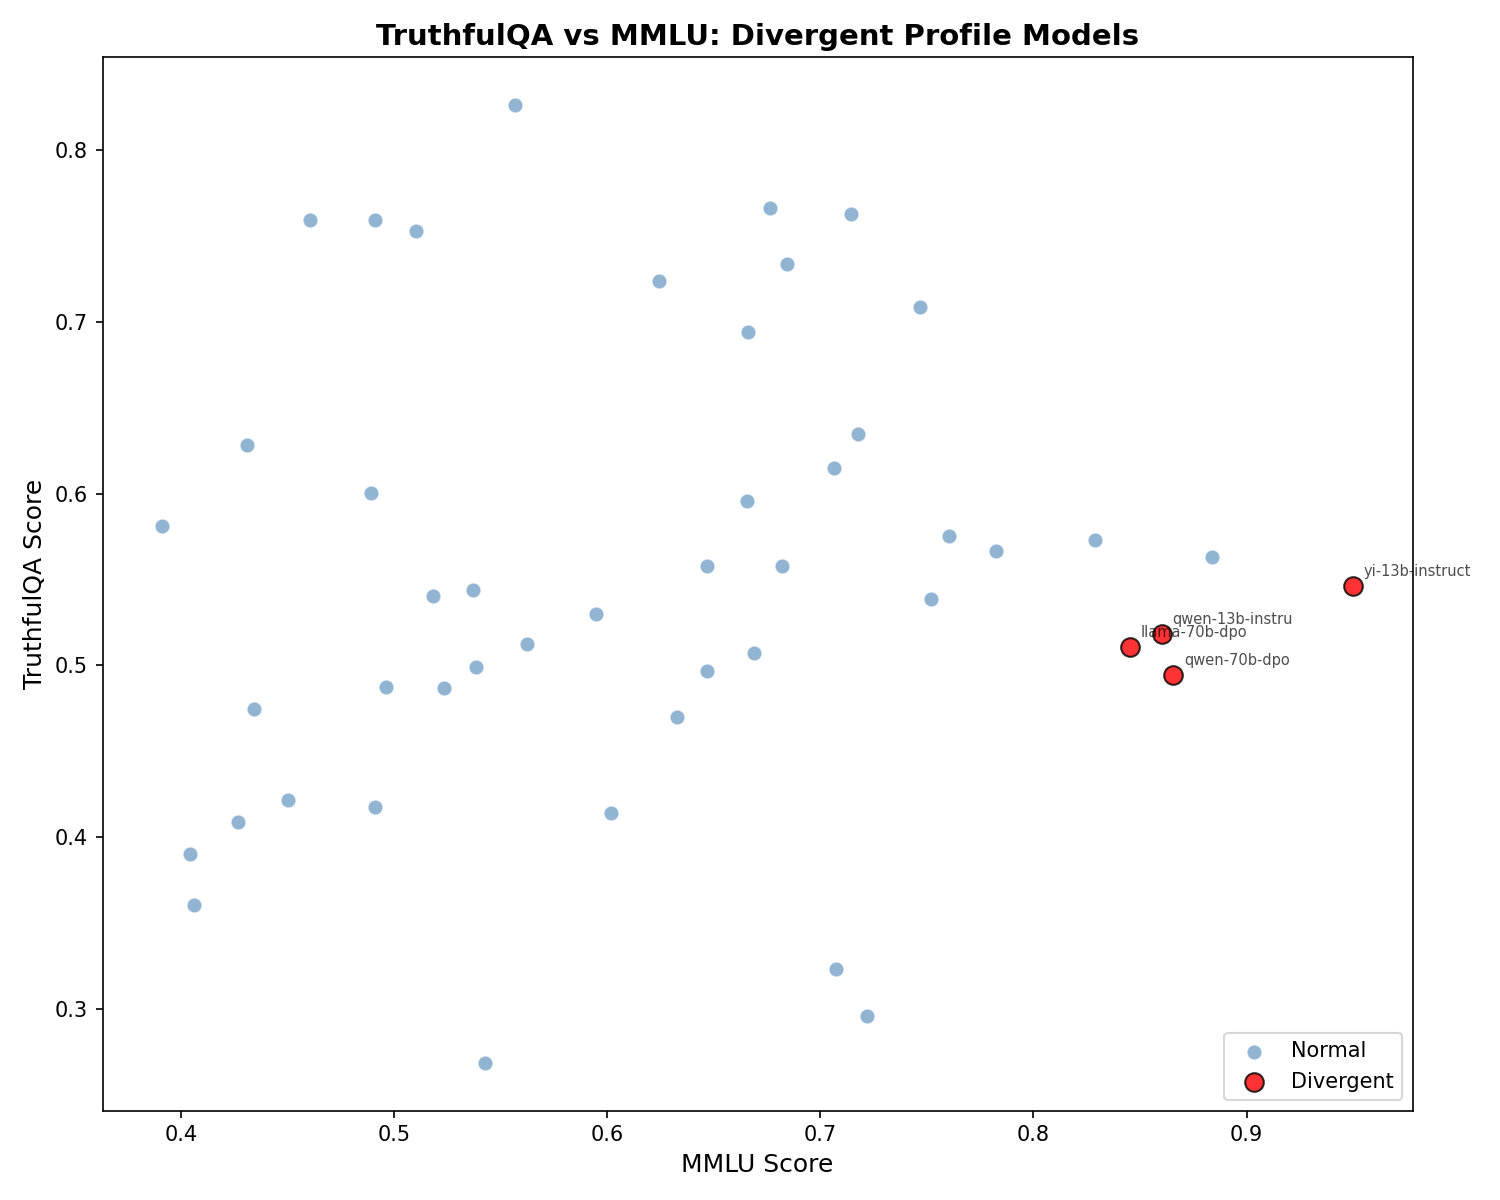
\includegraphics[width=\columnwidth]{figures/scatter_divergent.png}
\caption{Divergent Models Scatter}
\label{fig:scatter_divergent}
\end{figure}

\subsubsection{H-M2: HaluEval vs. TruthfulQA Distinctness}

HaluEval measures generation coherence, distinct from misconception resistance:

\begin{table}[htbp]
\centering
\resizebox{\columnwidth}{!}{%
\begin{tabular}{lll}
\toprule
Metric & Value & 95\% CI \\
\midrule
r(HaluEval, TruthfulQA) & 0.16 & [$-0.10$, 0.40] \\
r(intra-HaluEval, mean) & 0.65 & --- \\
\bottomrule
\end{tabular}
}
\end{table}

The cross-benchmark correlation (r=0.16, p=0.26) is not statistically significant, but the low magnitude satisfies the gate condition (r < 0.7).

\textbf{HaluEval subtask correlations with TruthfulQA:}

\begin{table}[htbp]
\centering
\resizebox{\columnwidth}{!}{%
\begin{tabular}{lll}
\toprule
Subtask & Spearman r & p-value \\
\midrule
QA & 0.15 & 0.29 \\
Dialogue & 0.15 & 0.31 \\
Summarization & 0.22 & 0.12 \\
\bottomrule
\end{tabular}
}
\end{table}

\textbf{Intra-HaluEval correlations:}

\begin{table}[htbp]
\centering
\resizebox{\columnwidth}{!}{%
\begin{tabular}{ll}
\toprule
Pair & Spearman r \\
\midrule
QA--Dialogue & 0.69 \\
QA--Summarization & 0.60 \\
Dialogue--Summarization & 0.64 \\
\bottomrule
\end{tabular}
}
\end{table}

The cross-benchmark correlation (r=0.16) is substantially lower than intra-HaluEval correlations (mean r=0.65).

\subsubsection{H-M3: FactScore Distinctness and Factor Structure}

FactScore measures a third distinct dimension:

\begin{table}[htbp]
\centering
\resizebox{\columnwidth}{!}{%
\begin{tabular}{llll}
\toprule
Correlation & Value & 95\% CI & p-value \\
\midrule
r(FactScore, TruthfulQA) & $-0.005$ & [$-0.27$, 0.26] & 0.97 \\
r(FactScore, HaluEval) & $-0.15$ & [$-0.41$, 0.13] & 0.31 \\
\bottomrule
\end{tabular}
}
\end{table}

Both correlations fall below 0.7 (near zero), passing the gate condition.

\textbf{PCA Results:}

\begin{table}[htbp]
\centering
\resizebox{\columnwidth}{!}{%
\begin{tabular}{ll}
\toprule
Metric & Value \\
\midrule
Components for 80\% variance & 3 \\
PC1 explained variance & 38.6\% \\
PC2 explained variance & 34.3\% \\
PC3 explained variance & 27.1\% \\
\bottomrule
\end{tabular}
}
\end{table}

\begin{figure}[htbp]
\centering
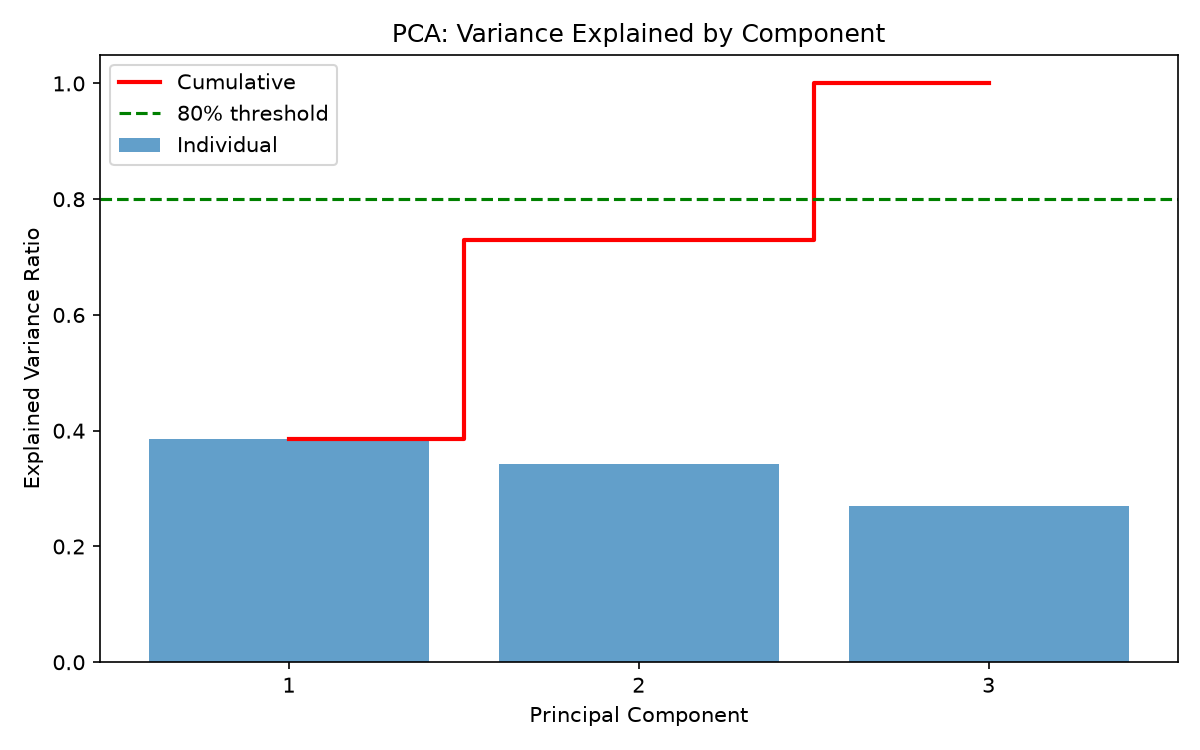
\includegraphics[width=\columnwidth]{figures/cumulative_variance.png}
\caption{PCA Cumulative Variance}
\label{fig:cumulative_variance}
\end{figure}

\subsubsection{Aggregate Results}

\begin{table}[htbp]
\centering
\resizebox{\columnwidth}{!}{%
\begin{tabular}{lll}
\toprule
Hypothesis & Gate & Result \\
\midrule
H-E1 & MUST\_WORK & PASS \\
H-M1 & MUST\_WORK & PASS \\
H-M2 & SHOULD\_WORK & PASS \\
H-M3 & SHOULD\_WORK & PASS \\
\bottomrule
\end{tabular}
}
\end{table}

All four hypotheses pass their gate conditions, supporting a three-dimensional truthfulness model.
